\section{Generalized Broyden tridiagonal function}
\label{sec:generalized_broyden_results}

The generalized Broyden tridiagonal function is defined as follows.
\begin{align}
F(x) &= \frac12 \sum_{i=1}^n f_k^2(x) &
f_k(x) &= (3-2x_k)x_k + 1 - x_{k-1} - x_{k+1}
\end{align}
Figure \ref{fig:generalized_broyden_surf} shows the surface plot of the 2-dimensional generalized Broyden tridiagonal function.
Notice that the area where the minimum lies is very flat, which makes it hard to converge to the minimum.

\begin{figure}
    \centering
    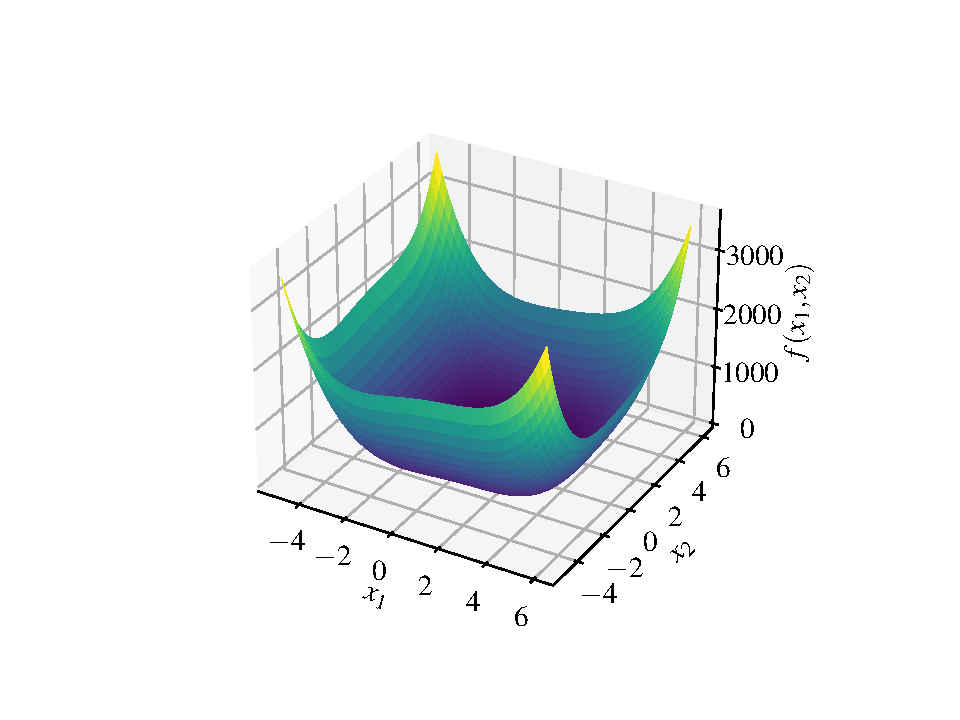
\includegraphics[width=0.5\textwidth]{figures/generalized_broyden_surf.pdf}
    \caption{Surface plot of the 2-dimensional generalized Broyden tridiagonal function}
    \label{fig:generalized_broyden_surf}
\end{figure}

\subsection{Exact gradient and Hessian}

The gradient of the generalized Broyden tridiagonal function is given by the following expression,
\begin{equation}
    \frac{\partial F}{\partial x_k} = \left \{ \begin{array}{ll}
    (3 - 4x_1)f_1(x) - f_2(x), & k = 1\\
    (3-4x_k)f_k(x) - f_{k+1}(x) - f_{k-1}(x), & 1 < k < n\\
    (3-4x_n)f_n(x) - f_{n-1}, & k = n
    \end{array} \right .
\end{equation}
computation can be eased considering that component $k$ depends only on $f_k$, $f_{k+1}$ and $f_{k-1}$.
The Hessian of the generalized Broyden tridiagonal function is given by the following expression.
\begin{equation}
    \frac{\partial^2 F}{\partial x_k \partial x_j} = \left \{ \begin{array}{ll}
    (3-4x_1)^2 - 4f_1(x) + 1, & k = j = 1 \\
    (3-4x_k)^2 - 4f_k(x) + 2, & 1 < k = j < n\\
    (3-4x_n)^2 - 4f_n(x) + 1, & k = j = n \\
    4x_k + 4x_{k+1} - 6, & |k-j| = 1\\
    1, & |k-j| = 2\\
    0, & \text{otherwise}
    \end{array} \right .
\end{equation}
Notice that the Hessian is a banded matrix, with only $n$ non-zero elements on the diagonal, $n-1$ non-zero elements on the first co-diagonal and $n-2$ non-zero elements on the second codiagonal.

\subsection{Finite differences gradient and Hessian}

When applying \ref{eq:findiff_gradient}, one can notice that the terms $F(x + he_k)$ and $F(x-he_k)$ only differ by terms $f_k$, $f_{k+1}$ and $f_{k-1}$.
Then to make function evaluations less expensive, we can define the following function $F_{\textit{fd},\,k}$, which can be plugged in \ref{eq:findiff_gradient} in place of $F$ yielding the same result.
\[
F_{\textit{fd},\,k}(x) = \frac12 f_k^2(x) + \frac12 f_{k+1}^2(x) + \frac12 f_{k-1}^2(x)
\]
The same procedure can be applied for the Hessian, considering that:
\begin{itemize}
    \item function evaluations to compute entry $h_{k,k}$ differ only by $f_k$, $f_{k+1}$ and $f_{k-1}$;
    \item function evaluation to compute entry $h_{k,k+1}$ differ only by $f_k$ and $f_{k+1}$;
    \item function evaluations to compute entry $h_{k,k+2}$ differ only by $f_{k-1}$.
\end{itemize}
Then to make function evaluations less expensive, we can define the functions $F_{\textit{fd},\,k,k}$, $F_{\textit{fd},\,k,k+1}$, $F_{\textit{fd},\,k,k+2}$, which can be plugged in \ref{eq:findiff_hessian} in place of $F$ yielding the same result to compute entries $h_{k,k}$, $h_{k,k+1}$ and $h_{k,k+2}$ respectively.
\begin{align*}
F_{\textit{fd},\,k,k}(x) &= \frac12 f_k^2(x) + \frac12 f_{k-1}^2(x) + \frac12 f_{k+1}^2(x)\\
F_{\textit{fd},\,k,k+1}(x) &= \frac12 f_k^2(x) + \frac12 f_{k+1}^2(x)\\
F_{\textit{fd},\,k,k+2}(x) &= \frac12 f_{k-1}^2(x)
\end{align*}
Carefully applying perturbations and properly defining some helper functions, computations for both gradient and Hessian can be vectorized, making the implementation efficient.